\documentclass{beamer}\usepackage[]{graphicx}\usepackage[]{xcolor}
% maxwidth is the original width if it is less than linewidth
% otherwise use linewidth (to make sure the graphics do not exceed the margin)
\makeatletter
\def\maxwidth{ %
  \ifdim\Gin@nat@width>\linewidth
    \linewidth
  \else
    \Gin@nat@width
  \fi
}
\makeatother

\definecolor{fgcolor}{rgb}{0.345, 0.345, 0.345}
\newcommand{\hlnum}[1]{\textcolor[rgb]{0.686,0.059,0.569}{#1}}%
\newcommand{\hlstr}[1]{\textcolor[rgb]{0.192,0.494,0.8}{#1}}%
\newcommand{\hlcom}[1]{\textcolor[rgb]{0.678,0.584,0.686}{\textit{#1}}}%
\newcommand{\hlopt}[1]{\textcolor[rgb]{0,0,0}{#1}}%
\newcommand{\hlstd}[1]{\textcolor[rgb]{0.345,0.345,0.345}{#1}}%
\newcommand{\hlkwa}[1]{\textcolor[rgb]{0.161,0.373,0.58}{\textbf{#1}}}%
\newcommand{\hlkwb}[1]{\textcolor[rgb]{0.69,0.353,0.396}{#1}}%
\newcommand{\hlkwc}[1]{\textcolor[rgb]{0.333,0.667,0.333}{#1}}%
\newcommand{\hlkwd}[1]{\textcolor[rgb]{0.737,0.353,0.396}{\textbf{#1}}}%
\let\hlipl\hlkwb

\usepackage{framed}
\makeatletter
\newenvironment{kframe}{%
 \def\at@end@of@kframe{}%
 \ifinner\ifhmode%
  \def\at@end@of@kframe{\end{minipage}}%
  \begin{minipage}{\columnwidth}%
 \fi\fi%
 \def\FrameCommand##1{\hskip\@totalleftmargin \hskip-\fboxsep
 \colorbox{shadecolor}{##1}\hskip-\fboxsep
     % There is no \\@totalrightmargin, so:
     \hskip-\linewidth \hskip-\@totalleftmargin \hskip\columnwidth}%
 \MakeFramed {\advance\hsize-\width
   \@totalleftmargin\z@ \linewidth\hsize
   \@setminipage}}%
 {\par\unskip\endMakeFramed%
 \at@end@of@kframe}
\makeatother

\definecolor{shadecolor}{rgb}{.97, .97, .97}
\definecolor{messagecolor}{rgb}{0, 0, 0}
\definecolor{warningcolor}{rgb}{1, 0, 1}
\definecolor{errorcolor}{rgb}{1, 0, 0}
\newenvironment{knitrout}{}{} % an empty environment to be redefined in TeX

\usepackage{alltt}
\usepackage{graphicx}

\usepackage{graphicx}
\usepackage{verbatim}
\usepackage{etoolbox}
\usepackage{everysel}
% \usepackage{enumitem}

%% This package allows text highlighting
\usepackage{soul}

%% This sets the theme of the presentation which controls
%% the formatting of the slides
\usetheme{Boadilla}

%% Turn off the navigation symbols
\setbeamertemplate{navigation symbols}{} 

%% Change the default itemize [ball]s to [circle]s
\setbeamertemplate{itemize items}[circle]

%% Change the default enumerate [ball]s to plain text
\setbeamertemplate{enumerate items}[default]

%% Load the enumitem package and ensure it works nicely with beamer
% \setitemize{label=\usebeamerfont*{itemize item}
%   \usebeamercolor[fg]{itemize item}
%   \usebeamertemplate{itemize item}}
% \setenumerate{label=\usebeamerfont*{enumerate item}
%   \usebeamercolor[fg]{enumerate item}
%   \usebeamertemplate{enumerate item}}

%% Set the author block so STATS 201/8 appears on every
\author{STATS 201/8}

%% Clear the date block
\date{}


\setbeamercolor{title}{bg=blue!40}
\setbeamerfont{title}{size=\LARGE,series=\bfseries}

%%Sectioning commands
\setbeamercolor{section title}{bg=blue!20}
\setbeamerfont{section title}{size=\large}

\setbeamertemplate{section page}{%
    \begingroup
        \begin{beamercolorbox}[sep=10pt,center,rounded=true,shadow=true]{section title}
        \usebeamerfont{section title}Section~\thechapter.\thesection \newline \insertsection\par
        \end{beamercolorbox}
		\vfill
    \endgroup
}

\newcommand{\BeginSection}[1]{\section{#1} \frame{\sectionpage}}
%\AtBeginSection[]{%
%    \begin{frame}
%        \sectionpage
%    \end{frame}
%}


%% This makes all equations blue
\AtBeginEnvironment{equation*}{\color{blue}}
\AtBeginEnvironment{align*}{\color{blue}}
\everymath{\color{blue}}

%% This puts a 0 point space between paragraphs, means we don't need to use vspace, or list environments if 
%% we don't want to
\setlength{\parskip}{0pt}


%% Russell: removes spaces after R input/output?
\setlength{\topsep}{0.5mm}

%% David: In addition to Russel's command to remove spaces after R input/output, these commands remove the space between R input/output.
%% Stackoverflow link: https://stackoverflow.com/questions/35734525/reduce-space-between-code-chunks-and-code-output-in-rmarkdown-beamer-presentatio
%% \setlength{\OuterFrameSep}{-2pt}
\makeatletter
\preto{\@verbatim}{\topsep=-1pt \partopsep=-1pt }
\makeatother

%% Some useful colors
\definecolor{darkgreen}{rgb}{0.176,0.486,0.031}
\definecolor{redbrown}{HTML}{950605}
\definecolor{darkred}{HTML}{d80605}


%% nice little macro for changing the font of R code
\newcommand{\rcode}[1]{\protect{\color{darkgreen}\texttt{#1}}}

%% macro for bold blue italics
\newcommand{\blueBoldEmph}[1]{{\color{blue}\textbf{\emph{#1}}}}

% ~iid macro
\newcommand{\iid }{\stackrel{iid}{\sim}}

%% Macro for t-test amd P-value
\newcommand{\ttest}{\emph{t}-test}
\newcommand{\pval}{\emph{P}-value}

%% Statistics operators 
\DeclareMathOperator{\Bias}{Bias}
\DeclareMathOperator{\Cov}{Cov}
\DeclareMathOperator*{\Cor}{Cor}
\DeclareMathOperator{\E}{E}
\DeclareMathOperator{\MSE}{MSE}
\DeclareMathOperator{\Odds}{Odds}
\DeclareMathOperator{\OR}{OR}
\DeclareMathOperator{\PMSE}{PMSE}
\DeclareMathOperator{\sd}{sd}
\DeclareMathOperator{\se}{se}
\DeclareMathOperator*{\Var}{Var}
\DeclareMathOperator{\logit}{logit}

%% Should see if can make this a mathop
\newcommand{\comb}[2]{\mbox{$\big(_{#2}^{#1}\big)$}}






\IfFileExists{upquote.sty}{\usepackage{upquote}}{}
\begin{document}
\newcommand{\thechapter}{9}

\title{Chapter 9: \\ Linear models with both numeric and factor explanatory variables \\~\\ Part 2: The model without interaction}
\institute{University of Auckland}


\begin{frame}
\titlepage
\end{frame}

\begin{frame}[t]
\frametitle{Learning Outcomes}
In this chapter you will learn about:
\begin{center}
\vspace{16pt}
\begin{minipage}{0.9\textwidth}
  \begin{itemize}
  \item More about linear models with both categorical and numeric explanatory variables
  \item Model selection using Occam's razor
  \item The \rcode{anova} function for joint hypothesis tests
  \item Fitting a model without an interaction term
  \item Interpretting fitted models with factors having more than two levels 
  \item Changing the reference level of a categorical variable
  \item Relevant \rcode{R}-code.
  \end{itemize}
\end{minipage}
\end{center}
\end{frame}


%%%%%%%%%%%%%%%%%%%%%%%%%%%%%%%%%%%%%%%%%%%%%%%%%%%%%%%%%%%%%%%%%%%%%%%%%%%%%%%%%%%%%%%%%%%
\BeginSection{Example: Using both IQ and teaching method to explain increase in language proficiency}
%%%%%%%%%%%%%%%%%%%%%%%%%%%%%%%%%%%%%%%%%%%%%%%%%%%%%%%%%%%%%%%%%%%%%%%%%%%%%%%%%%%%%%%%%%%


\begin{frame}
\frametitle{Student language score by teaching method and IQ}
In the following example, educational experts were interested in which of three different teaching methods was most effective in increasing a language score for students of a range of abilities -- as measured by IQ.\\
\bigskip 
In order to do this, 
30 students were randomly allocated into three groups and each group was taught using a different teaching method. 
Each student's IQ was measured before the teaching programme began. \\
\bigskip 
This randomisation was done to ensure that a range of student abilities was represented in each group. As students were in a test environment we can assume that their test scores are independent of each other.\\

\bigskip
The variables measured were:
\medskip

\begin{tabular}{lp{15cm}}
  \rcode{lang} & the language test score achieved by the student after instruction\\
	\rcode{IQ}	& the student's IQ\\
	\rcode{method} &	the teaching method used (1, 2 or 3) 
\end{tabular}

\end{frame}


\begin{frame}[fragile]
\frametitle{Student language score by  teaching method and IQ\ldots}
It was of interest to see if there was any difference in the students' expected language score between teaching methods, and if this difference depended on IQ.
\medskip

As usual, we begin by inspecting the data:

\begin{knitrout}\scriptsize
\definecolor{shadecolor}{rgb}{0.969, 0.969, 0.969}\color{fgcolor}\begin{kframe}
\begin{alltt}
\hlstd{> }\hlcom{## Invoke the s20x library}
\hlstd{> }\hlkwd{library}\hlstd{(s20x)}
\hlstd{> }\hlcom{## Importing data found in the s20x library into R}
\hlstd{> }\hlkwd{data}\hlstd{(teach.df)}
\hlstd{> }\hlcom{## Plot the data with trendscatter()}
\hlstd{> }\hlkwd{trendscatter}\hlstd{(lang} \hlopt{~} \hlstd{IQ,} \hlkwc{f} \hlstd{=} \hlnum{0.8}\hlstd{,} \hlkwc{ylim} \hlstd{=} \hlkwd{c}\hlstd{(}\hlnum{40}\hlstd{,} \hlnum{110}\hlstd{),} \hlkwc{data} \hlstd{= teach.df,}
\hlstd{+ }             \hlkwc{ylab}\hlstd{=}\hlstr{"Language score"}\hlstd{)}
\hlstd{> }\hlcom{## Note that f is the proportion of points in the plot which influence the}
\hlstd{> }\hlcom{## smooth at each value. Larger values of f give more smoothness!}
\end{alltt}
\end{kframe}
\end{knitrout}

\end{frame}

\begin{frame}[fragile]
\frametitle{Student language score by teaching method and IQ\ldots}


\begin{figure}
  \centering
  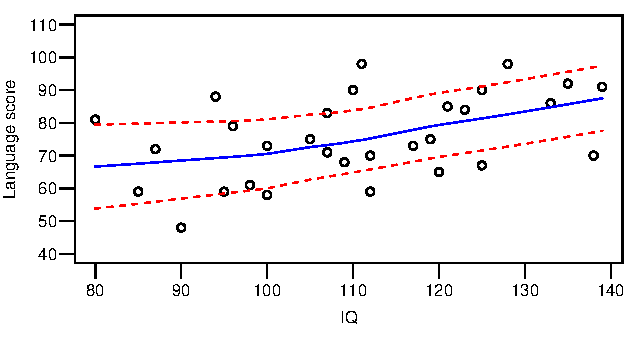
\includegraphics{figure/RC-H09-002}
\end{figure}

Hmmm -- positive relationship with IQ suggested, but statistical significance not obvious. A plot that shows the teaching method would be more useful.
\end{frame}


\begin{frame}[fragile]
\frametitle{Student language score by teaching method and IQ\ldots}
In dataframe \rcode{teach.df} the \rcode{method} is recorded as a number, 1, 2 or 3. 
\begin{knitrout}\scriptsize
\definecolor{shadecolor}{rgb}{0.969, 0.969, 0.969}\color{fgcolor}\begin{kframe}
\begin{alltt}
\hlstd{> }\hlstd{teach.df}\hlopt{$}\hlstd{method}
\end{alltt}
\begin{verbatim}
 [1] 1 1 1 1 1 1 1 1 1 1 2 2 2 2 2 2 2 2 2 2 3 3 3 3 3 3 3 3 3 3
\end{verbatim}
\begin{alltt}
\hlstd{> }\hlkwd{class}\hlstd{(teach.df}\hlopt{$}\hlstd{method)}
\end{alltt}
\begin{verbatim}
[1] "integer"
\end{verbatim}
\end{kframe}
\end{knitrout}

However, these are just labels and could as easily have been "A", "B" or "C".
So, \rcode{method} needs to be `coerced' into a factor so that it does not 
get treated as a numeric variable\footnote{What would happen if \rcode{lm} was treated \rcode{method} as numeric???}.\\
\medskip
\begin{knitrout}\scriptsize
\definecolor{shadecolor}{rgb}{0.969, 0.969, 0.969}\color{fgcolor}\begin{kframe}
\begin{alltt}
\hlstd{> }\hlstd{teach.df}\hlopt{$}\hlstd{method} \hlkwb{=} \hlkwd{factor}\hlstd{(teach.df}\hlopt{$}\hlstd{method)}
\hlstd{> }\hlstd{teach.df}\hlopt{$}\hlstd{method}
\end{alltt}
\begin{verbatim}
 [1] 1 1 1 1 1 1 1 1 1 1 2 2 2 2 2 2 2 2 2 2 3 3 3 3 3 3 3 3 3 3
Levels: 1 2 3
\end{verbatim}
\begin{alltt}
\hlstd{> }\hlkwd{class}\hlstd{(teach.df}\hlopt{$}\hlstd{method)}
\end{alltt}
\begin{verbatim}
[1] "factor"
\end{verbatim}
\end{kframe}
\end{knitrout}
\medskip
Not much has changed, but when we use \rcode{method} as the explanatory variable,
plot functions and \rcode{lm} will now do the right thing since it is now a factor variable.
\end{frame}



\begin{frame}[fragile]
\frametitle{Student language score by teaching method and IQ\ldots}
\begin{knitrout}\scriptsize
\definecolor{shadecolor}{rgb}{0.969, 0.969, 0.969}\color{fgcolor}\begin{kframe}
\begin{alltt}
\hlstd{> }\hlkwd{plot}\hlstd{(lang} \hlopt{~} \hlstd{method,} \hlkwc{ylim}\hlstd{=}\hlkwd{c}\hlstd{(}\hlnum{40}\hlstd{,}\hlnum{110}\hlstd{),} \hlkwc{data}\hlstd{=teach.df,} \hlkwc{ylab}\hlstd{=}\hlstr{"Language score"}\hlstd{)}
\end{alltt}
\end{kframe}
\end{knitrout}



\begin{figure}
  \centering
  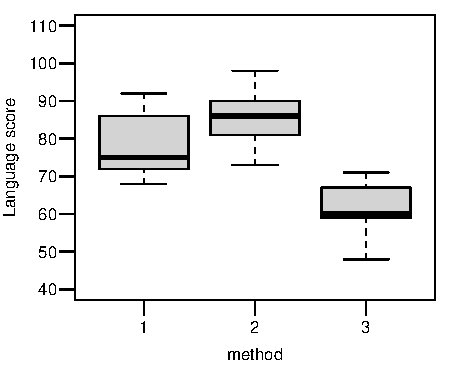
\includegraphics{figure/RC-H09-005}
\end{figure}

Teaching method 2 seems best. The worst appears to be method 3.

\end{frame}



\begin{frame}[fragile]
\frametitle{Student language score by teaching method and IQ\ldots}
A more useful plot:
\begin{knitrout}\scriptsize
\definecolor{shadecolor}{rgb}{0.969, 0.969, 0.969}\color{fgcolor}\begin{kframe}
\begin{alltt}
\hlstd{> }\hlkwd{plot}\hlstd{(lang} \hlopt{~} \hlstd{IQ,} \hlkwc{ylim}\hlstd{=}\hlkwd{c}\hlstd{(}\hlnum{40}\hlstd{,}\hlnum{110}\hlstd{),} \hlkwc{pch}\hlstd{=}\hlkwd{as.character}\hlstd{(method),} \hlkwc{data} \hlstd{= teach.df,}
\hlstd{+ }     \hlkwc{ylab}\hlstd{=}\hlstr{"Language score"}\hlstd{)}
\end{alltt}
\end{kframe}
\end{knitrout}

%plot(lang ~ IQ, ylim=c(40,110), pch=as.character(method), data = teach.df,
%     ylab="Language score",col=c("red","blue","green")[method])




\begin{figure}
  \centering
  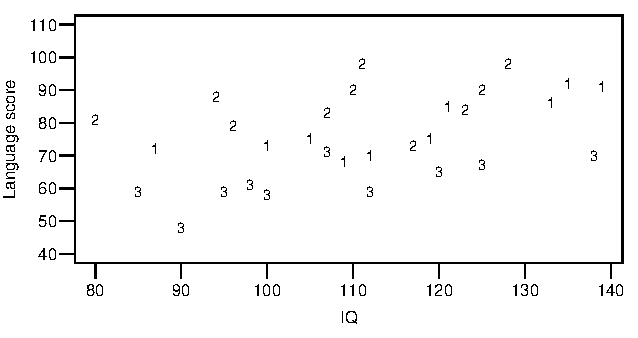
\includegraphics{figure/RC-H09-007}
\end{figure}

What do you see in this plot?

\end{frame}
 
 
 
\begin{frame}[fragile]
\frametitle{Student language score by  teaching method and IQ\ldots}

What we see here is that the data for methods 1, 2, 3 seem to be scattered around approximately parallel straight lines. This means the \rcode{IQ} effect appears the same regardless of the teaching method. Conversely, the \rcode{Method} effect appears to be the same regardless of IQ. \\
\bigskip

In other words, it looks like \rcode{IQ} and \rcode{method} {\bf do not} interact, i.e., there is no need to complicate the model by using a different slope for each method.  \\
\bigskip 
When we look at this data we see that the method 2 students are (on average) doing considerably better than method 1 students,  who are (on average) better than the method 3 students.\\
\bigskip
So, we suspect that we there may be a difference in the expected teaching scores between methods, and that the effect of IQ may be the same regardless of method. We'll need to   fit an appropriate linear model to find out for sure.\\
\end{frame}




\begin{frame}[fragile]
\frametitle{Student language score by  teaching method and IQ\ldots}
\framesubtitle{Fitting and checking the interaction model}
We will fit the model with interaction first, anticipating that the interaction will not be significant.\\
\medskip
Here goes\ldots, along with the usual assumption checks.\\
\medskip
\begin{knitrout}\scriptsize
\definecolor{shadecolor}{rgb}{0.969, 0.969, 0.969}\color{fgcolor}\begin{kframe}
\begin{alltt}
\hlstd{> }\hlstd{TeachIQmethod.fit}\hlkwb{=}\hlkwd{lm}\hlstd{(lang}\hlopt{~}\hlstd{IQ}\hlopt{*}\hlstd{method,} \hlkwc{data}\hlstd{=teach.df)}
\hlstd{> }\hlkwd{plot}\hlstd{(TeachIQmethod.fit,} \hlkwc{which} \hlstd{=} \hlnum{1}\hlstd{)}
\end{alltt}
\end{kframe}
\end{knitrout}


\begin{figure}
  \centering
  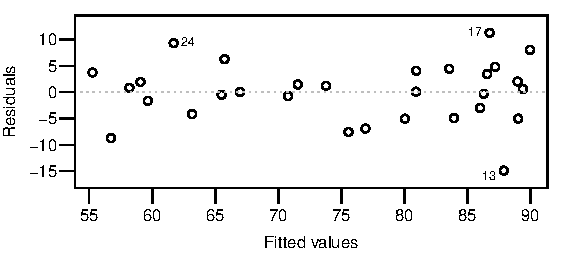
\includegraphics{figure/RC-H09-009}
\end{figure}

The \textbf{EOV} and no-trend assumptions seem to be okay.
\end{frame}


\begin{frame}[fragile]
\frametitle{Student language score by  teaching method and IQ\ldots}
\framesubtitle{Fitting and checking the interaction model\ldots}
\begin{knitrout}\scriptsize
\definecolor{shadecolor}{rgb}{0.969, 0.969, 0.969}\color{fgcolor}\begin{kframe}
\begin{alltt}
\hlstd{> }\hlkwd{normcheck}\hlstd{(TeachIQmethod.fit)}
\end{alltt}
\end{kframe}
\end{knitrout}



\begin{figure}
  \centering
  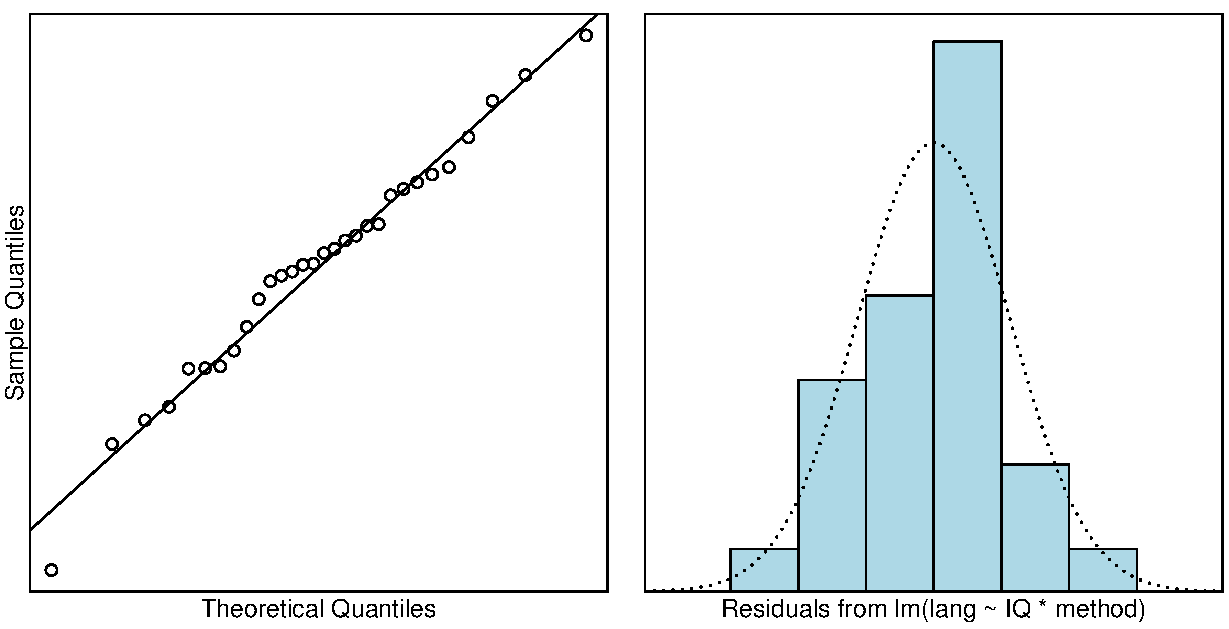
\includegraphics[scale=0.5]{figure/RC-H09-011}
\end{figure}  

\end{frame}


\begin{frame}[fragile]
\frametitle{Student language score by  teaching method and IQ\ldots}
\framesubtitle{Fitting and checking the interaction model\ldots}
\begin{knitrout}\scriptsize
\definecolor{shadecolor}{rgb}{0.969, 0.969, 0.969}\color{fgcolor}\begin{kframe}
\begin{alltt}
\hlstd{> }\hlkwd{cooks20x}\hlstd{(TeachIQmethod.fit)}
\end{alltt}
\end{kframe}
\end{knitrout}



\begin{figure}
  \centering
  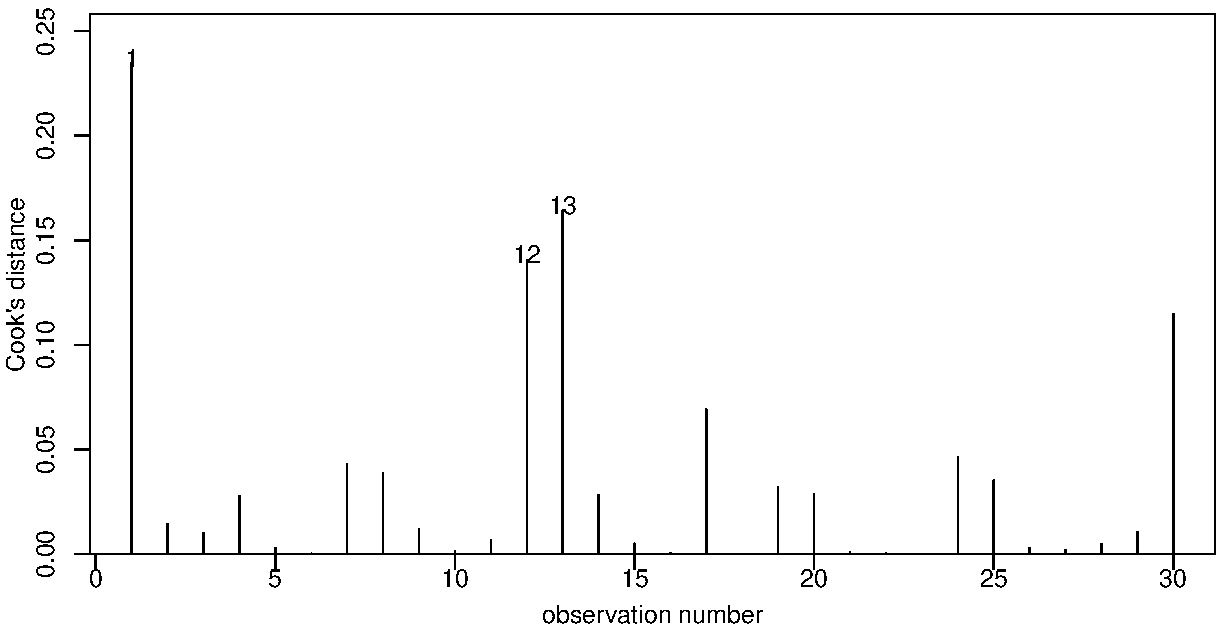
\includegraphics[scale=0.5]{figure/RC-H09-013}
\end{figure}

It looks like we can trust the output of the fitted model.
\end{frame}




%%%%%%%%%%%%%%%%%%%%%%%%%%%%%%%%%%%%%%%%%%%%%%%%%%%%%%%%%%%%%%%%%%%%%%%%%%%%%%%%%%%%%%%%%%%
\BeginSection{Model selection using Occam's razor}
%%%%%%%%%%%%%%%%%%%%%%%%%%%%%%%%%%%%%%%%%%%%%%%%%%%%%%%%%%%%%%%%%%%%%%%%%%%%%%%%%%%%%%%%%%%



\begin{frame}[fragile]
\frametitle{Student language score by  teaching method and IQ\ldots}
\framesubtitle{The fitted interaction model}
Our fitted interaction model is:
\bigskip

\begin{knitrout}\scriptsize
\definecolor{shadecolor}{rgb}{0.969, 0.969, 0.969}\color{fgcolor}\begin{kframe}
\begin{alltt}
\hlstd{> }\hlkwd{summary}\hlstd{(TeachIQmethod.fit)}
\end{alltt}
\end{kframe}
\end{knitrout}

\begin{knitrout}\scriptsize
\definecolor{shadecolor}{rgb}{0.969, 0.969, 0.969}\color{fgcolor}\begin{kframe}
\begin{verbatim}
Coefficients:
            Estimate Std. Error t value Pr(>|t|)   
(Intercept)  26.8346    14.5250   1.847  0.07704 . 
IQ            0.4471     0.1241   3.604  0.00142 **
method2      39.0098    20.7473   1.880  0.07227 . 
method3       3.5617    19.7222   0.181  0.85820   
IQ:method2   -0.2587     0.1831  -1.413  0.17042   
IQ:method3   -0.1546     0.1749  -0.883  0.38574   
---
Residual standard error: 6.199 on 24 degrees of freedom
Multiple R-squared:  0.8121,	Adjusted R-squared:  0.7729 
F-statistic: 20.74 on 5 and 24 DF,  p-value: 5.284e-08
\end{verbatim}
\end{kframe}
\end{knitrout}
\vfill
\end{frame}



\begin{frame}[fragile]
\frametitle{Model selection using Occam's razor}
In previous Chapters we've seen that we remove terms that are not significant if doing so simplifies the fitted model. This is a very important principle of model selection and is an application of the ``principle of parsimony'', also known as \textbf{Occam's Razor}.\footnote{Named after William of Ockham (c. 1287-1347), who was an English Franciscan friar and scholastic philosopher and theologian.} :
\medskip

``The principle states that among competing models that predict equally well, the one with the fewest parameters should be selected."
\medskip

In STATS20x we sometimes call it the \textbf{KISS} principle -- ``keep it simple, statistician".
\bigskip

In this class the general model selection approach we use is to do a hypothesis test to determine if we can remove the most complicated term from our current model.\footnote{In STATS 330 you will several holistic approaches to model selection that are based on the estimated predictive ability of the model.}
\end{frame}


\begin{frame}[fragile]
\frametitle{Student language score by teaching method and IQ\ldots}
\framesubtitle{Model selection using Occam's razor}
In our above interaction model for language score, the interaction term is the most complicated term, so we need to test whether the interaction is significant.
\bigskip

Hmmm, the null hypothesis of no interaction is saying that the last two coefficients in the summary table are both zero. That is, $H_0: \beta_4=\beta_5=0$.\footnote{A hypothesis that specifies the value of two or more coefficients is called a {\bf joint} hypothesis.}\\
\bigskip

To do a single test about whether two or more coefficients are zero we need to produce an ANOVA table, using the \rcode{anova} function.
\vfill
\end{frame}


\begin{frame}[fragile]
\frametitle{Student language score by  teaching method and IQ\ldots}
\framesubtitle{Model selection using Occam's razor\ldots}
\begin{knitrout}\scriptsize
\definecolor{shadecolor}{rgb}{0.969, 0.969, 0.969}\color{fgcolor}\begin{kframe}
\begin{alltt}
\hlstd{> }\hlkwd{anova}\hlstd{(TeachIQmethod.fit)}
\end{alltt}
\begin{verbatim}
Analysis of Variance Table

Response: lang
          Df  Sum Sq Mean Sq F value    Pr(>F)    
IQ         1 1004.42 1004.42 26.1416 3.124e-05 ***
method     2 2901.83 1450.91 37.7625 3.867e-08 ***
IQ:method  2   78.82   39.41  1.0257    0.3737    
Residuals 24  922.13   38.42                      
---
Signif. codes:  0 '***' 0.001 '**' 0.01 '*' 0.05 '.' 0.1 ' ' 1
\end{verbatim}
\end{kframe}
\end{knitrout}
The \pval{} associated with the interaction term \rcode{IQ:method} is large. 
So we conclude we do not have evidence of an interaction.
\medskip

This means we do not need to compute a different slope for each teaching method -- just different intercepts. Our instincts were right. 
This saves us having to have an extra two parameters in our final model, and simplifies the interpretation of our model since the lines are parallel.

\end{frame}



\begin{frame}[fragile]
\frametitle{Understanding the ANOVA table}

An \rcode{anova} table is  based on partitioning the total sums of squares, TSS. Recall, this is the residual sums of squares of the null model. The TSS is given by summing the values in the \rcode{Sum sq} column of the table.
\bigskip

In the above table, TSS $=1004.42+2901.83+78.82+922.13=4907.2$. The amount of unexplained variability in our fitted model is given by the \rcode{Residuals} value of 922.13. This means that $922.13/4907.2=0.188$ is the proportion of the total variability that is not explained. The $R^2$ is therefore $1-0.188=0.812$.
\bigskip \bigskip

Now, back to our example, where we now need to consider the formulation of the parallel line model.
\end{frame}



\begin{frame}[fragile]
\frametitle{Student language score by  teaching method and IQ\ldots}
\framesubtitle{Fitting the model without interaction}
Occam's razor dictates that we sharpen our model by removing the interaction term.
To do this, we simply replace \rcode{*} by \rcode{+} in the model formula.\\

Non-interaction models are sometimes referred to as \emph{additive models} (as the effects `add up'),
or `main effects' models.

\begin{knitrout}\scriptsize
\definecolor{shadecolor}{rgb}{0.969, 0.969, 0.969}\color{fgcolor}\begin{kframe}
\begin{alltt}
\hlstd{> }\hlstd{TeachIQmethod.fit2}\hlkwb{=}\hlkwd{lm}\hlstd{(lang}\hlopt{~}\hlstd{IQ}\hlopt{+}\hlstd{method,} \hlkwc{data}\hlstd{=teach.df)}
\hlstd{> }\hlkwd{summary}\hlstd{(TeachIQmethod.fit2)}
\end{alltt}
\end{kframe}
\end{knitrout}

\begin{knitrout}\scriptsize
\definecolor{shadecolor}{rgb}{0.969, 0.969, 0.969}\color{fgcolor}\begin{kframe}
\begin{verbatim}
Coefficients:
             Estimate Std. Error t value Pr(>|t|)    
(Intercept)  42.08552    8.73921   4.816 5.47e-05 ***
IQ            0.31564    0.07341   4.299 0.000213 ***
method2       9.87793    2.82068   3.502 0.001688 ** 
method3     -14.15922    2.85240  -4.964 3.70e-05 ***
---
Residual standard error: 6.205 on 26 degrees of freedom
Multiple R-squared:  0.796,	Adjusted R-squared:  0.7725 
F-statistic: 33.82 on 3 and 26 DF,  p-value: 3.986e-09
\end{verbatim}
\end{kframe}
\end{knitrout}

All the assumptions are fine (not shown) -- not surprising, as all we have done is remove
a term that was not significant.
\end{frame}



\begin{frame}[fragile]
\frametitle{Student language score by teaching method and IQ\ldots}
\framesubtitle{Interpretting the no-interaction model}
The equation for the parallel lines (i.e, no-interaction) model is
\[
\rcode{lang}=\beta_0+\beta_1 \times \rcode{IQ}+\beta_{2} \times \rcode{D2} +\beta_{3} \times \rcode{D3} +\varepsilon
\]
where, as usual $\varepsilon \iid N(0, \sigma^2)$.

There are two indicator variables since teaching method has three levels:
\begin{itemize}
\item \rcode{D2} is an indicator variable whereby: \rcode{D2 = 1} if teaching method 2 is taught -- otherwise it is 0.
\item \rcode{D3} is an indicator variable whereby: \rcode{D3 = 1} if teaching method 3 is taught -- otherwise it is 0.
\item Teaching method 1 is the \textbf{reference/baseline} level group. 
\end{itemize}
\medskip 

\hl{$\beta_{2}$} and \hl{$\beta_{3}$} represent the change in expected score 
(for any fixed student IQ)
when we compare teaching method 2 or 3 to teaching method 1 (baseline).
\end{frame}



\begin{frame}[fragile] 
\frametitle{Student language score by  teaching method and IQ\ldots}
\framesubtitle{Model selection using Occam's razor\ldots}
The KISS principle requires us to determine if we can further simplify our model. 
\medskip

The no-interaction model can be simplified by removing the \rcode{IQ} term and/or the \rcode{method} terms. We see immediately from the summary table that \rcode{IQ} is highly significant, and so should not be removed.
\medskip

To see if the \rcode{method} terms can be removed we want to test the joint null hypothesis that the intercepts are all identical, $H_0: \beta_2=\beta_3=0$.
This would simplify our model to a simple linear regression model.
\bigskip

\textbf{Recall:} 
To do a test about whether two or more coefficients are zero we need to produce an 
ANOVA table, using the \rcode{anova} function.
\vfill
\end{frame}



\begin{frame}[fragile, label={anova1}]
\frametitle{Student language score by  teaching method and IQ\ldots}
\framesubtitle{Model selection using Occam's razor\ldots}
Let us see if we really do have identical intercepts.  \\
\medskip
\begin{knitrout}\scriptsize
\definecolor{shadecolor}{rgb}{0.969, 0.969, 0.969}\color{fgcolor}\begin{kframe}
\begin{alltt}
\hlstd{> }\hlkwd{anova}\hlstd{(TeachIQmethod.fit2)}
\end{alltt}
\begin{verbatim}
Analysis of Variance Table

Response: lang
          Df Sum Sq Mean Sq F value    Pr(>F)    
IQ         1 1004.4  1004.4  26.090 2.529e-05 ***
method     2 2901.8  1450.9  37.688 2.077e-08 ***
Residuals 26 1001.0    38.5                      
---
Signif. codes:  0 '***' 0.001 '**' 0.01 '*' 0.05 '.' 0.1 ' ' 1
\end{verbatim}
\end{kframe}
\end{knitrout}
\medskip
The \pval{} associated with the \rcode{method} term is very small, so we conclude that the intercepts are different.\\
\medskip
We do have to fit different intercepts for each teaching method. Our instincts were right.
\end{frame}


\begin{frame}[fragile]
\frametitle{Student language score by  teaching method and IQ\ldots}
\framesubtitle{Our preferred model}
Our preferred model is the no-interaction model:

\begin{knitrout}\scriptsize
\definecolor{shadecolor}{rgb}{0.969, 0.969, 0.969}\color{fgcolor}\begin{kframe}
\begin{alltt}
\hlstd{> }\hlkwd{summary}\hlstd{(TeachIQmethod.fit2)}
\end{alltt}
\end{kframe}
\end{knitrout}

\begin{knitrout}\scriptsize
\definecolor{shadecolor}{rgb}{0.969, 0.969, 0.969}\color{fgcolor}\begin{kframe}
\begin{verbatim}
Coefficients:
             Estimate Std. Error t value Pr(>|t|)    
(Intercept)  42.08552    8.73921   4.816 5.47e-05 ***
IQ            0.31564    0.07341   4.299 0.000213 ***
method2       9.87793    2.82068   3.502 0.001688 ** 
method3     -14.15922    2.85240  -4.964 3.70e-05 ***
---
Residual standard error: 6.205 on 26 degrees of freedom
Multiple R-squared:  0.796,	Adjusted R-squared:  0.7725 
F-statistic: 33.82 on 3 and 26 DF,  p-value: 3.986e-09
\end{verbatim}
\end{kframe}
\end{knitrout}
\vfill
\end{frame}



\begin{frame}[fragile]
\frametitle{Student language score by teaching method and IQ\ldots}
\framesubtitle{The fitted model}
\begin{knitrout}\scriptsize
\definecolor{shadecolor}{rgb}{0.969, 0.969, 0.969}\color{fgcolor}\begin{kframe}
\begin{alltt}
\hlstd{> }\hlkwd{plot}\hlstd{(lang} \hlopt{~} \hlstd{IQ,} \hlkwc{ylim}\hlstd{=}\hlkwd{c}\hlstd{(}\hlnum{40}\hlstd{,}\hlnum{110}\hlstd{),} \hlkwc{pch}\hlstd{=}\hlkwd{as.character}\hlstd{(method),} \hlkwc{data} \hlstd{= teach.df,}
\hlstd{+ }     \hlkwc{ylab}\hlstd{=}\hlstr{"Language score"}\hlstd{)}
\hlstd{> }\hlstd{b} \hlkwb{=} \hlkwd{coef}\hlstd{(TeachIQmethod.fit2)}
\hlstd{> }\hlkwd{abline}\hlstd{(b[}\hlnum{1}\hlstd{], b[}\hlnum{2}\hlstd{],} \hlkwc{lty} \hlstd{=} \hlnum{2}\hlstd{,} \hlkwc{col} \hlstd{=} \hlstr{"darkorange"}\hlstd{)}
\hlstd{> }\hlkwd{abline}\hlstd{(b[}\hlnum{1}\hlstd{]} \hlopt{+} \hlstd{b[}\hlnum{3}\hlstd{], b[}\hlnum{2}\hlstd{],} \hlkwc{lty} \hlstd{=} \hlnum{2}\hlstd{,} \hlkwc{col} \hlstd{=} \hlstr{"tomato"}\hlstd{)}
\hlstd{> }\hlkwd{abline}\hlstd{(b[}\hlnum{1}\hlstd{]} \hlopt{+} \hlstd{b[}\hlnum{4}\hlstd{], b[}\hlnum{2}\hlstd{],} \hlkwc{lty} \hlstd{=} \hlnum{2}\hlstd{,} \hlkwc{col} \hlstd{=} \hlstr{"steelblue"}\hlstd{)}
\end{alltt}
\end{kframe}
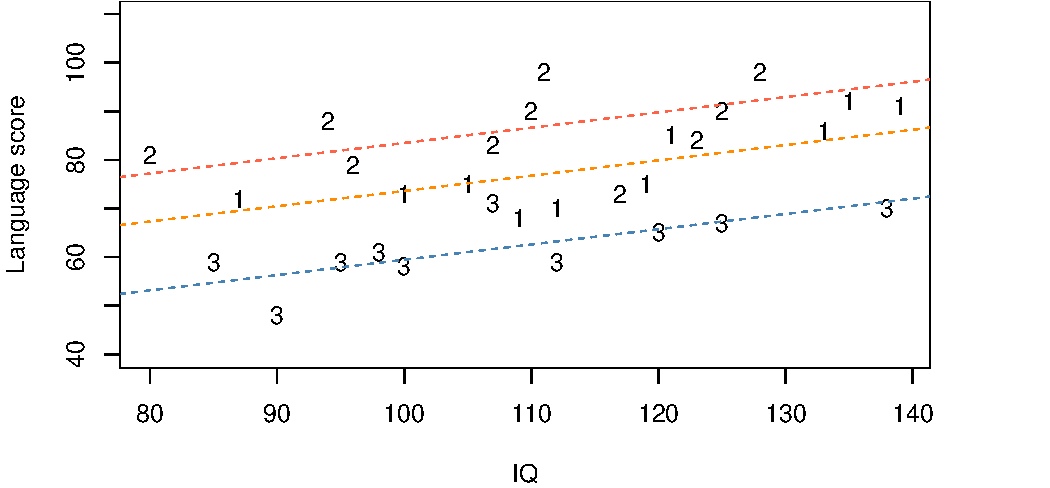
\includegraphics[width=\maxwidth]{figure/RC-H09-0022b-1} 
\end{knitrout}
\end{frame}



\begin{frame}[fragile]
\frametitle{Student language score by teaching method and IQ\ldots}
\framesubtitle{Interpreting the output\ldots}
We are now able to deduce:
\bigskip
\begin{itemize}
\item $\beta_1>0$ $\implies$\footnote{ $\implies$ means \emph{implies that}.} \rcode{IQ} has a common positive effect on the expected language score of all students
\item $\beta_{2}>0$ $\implies$ teaching method 2  is better than teaching method 1 regardless of a student's \rcode{IQ}.
\item $\beta_{3}< 0$ $\implies$ teaching method 3 is worse than teaching method 1 regardless of a student's \rcode{IQ}.
\end{itemize}
\bigskip
Our initial hunch about the best model has been justified.
\end{frame}


%%%%%%%%%%%%%%%%%%%%%%%%%%%%%%%%%%%%%%%%%%%%%%%%%%%%%%%%%%%%%%%%%%%%%%%%%%%%%%%%%%%%%%%%%%%
\BeginSection{Changing the reference level of teaching method}
%%%%%%%%%%%%%%%%%%%%%%%%%%%%%%%%%%%%%%%%%%%%%%%%%%%%%%%%%%%%%%%%%%%%%%%%%%%%%%%%%%%%%%%%%%%


\begin{frame}[fragile]
\frametitle{Student language score by  teaching method and IQ\ldots}
\framesubtitle{Changing the reference level}
The above statements are useful, but are incomplete -- we still don't know how method 2 differs from method 3?\footnote{The issue of estimating all pairwise differences between factor levels is an issue we deal with more
fully in a later chapter.}\\
\bigskip
The \rcode{lm} function has chosen the baseline (i.e., reference) level to be method 1 since ``1'' comes before ``2'' and ``3'' when these values are sorted by a computer.
We need to change this to make method 2 (or alternatively method 3) the baseline.
The fitted model will be exactly the same, but the intercept coefficients will change due to the change in reference level. \\
\bigskip
Here is the \rcode{R} code to do this:\\
\medskip

\begin{knitrout}\scriptsize
\definecolor{shadecolor}{rgb}{0.969, 0.969, 0.969}\color{fgcolor}\begin{kframe}
\begin{alltt}
\hlstd{> }\hlstd{teach.df}\hlopt{$}\hlstd{method} \hlkwb{=} \hlkwd{relevel}\hlstd{(teach.df}\hlopt{$}\hlstd{method,} \hlkwc{ref} \hlstd{=} \hlstr{"2"}\hlstd{)}
\hlstd{> }\hlstd{TeachIQmethod.fit3}\hlkwb{=}\hlkwd{lm}\hlstd{(lang}\hlopt{~}\hlstd{IQ}\hlopt{+}\hlstd{method,} \hlkwc{data}\hlstd{=teach.df)}
\end{alltt}
\end{kframe}
\end{knitrout}

Let us compare the \rcode{summary}s of \rcode{TeachIQmethod.fit3} and \rcode{TeachIQmethod.fit2}.
\end{frame}


\begin{frame}[fragile]
\frametitle{Student language score by  teaching method and IQ\ldots}
\framesubtitle{Interpreting the output}
\begin{knitrout}\scriptsize
\definecolor{shadecolor}{rgb}{0.969, 0.969, 0.969}\color{fgcolor}\begin{kframe}
\begin{alltt}
\hlstd{> }\hlkwd{summary}\hlstd{(TeachIQmethod.fit3)}
\end{alltt}
\end{kframe}
\end{knitrout}
\begin{knitrout}\scriptsize
\definecolor{shadecolor}{rgb}{0.969, 0.969, 0.969}\color{fgcolor}\begin{kframe}
\begin{verbatim}
Coefficients:
             Estimate Std. Error t value Pr(>|t|)    
(Intercept)  51.96345    8.24637   6.301 1.14e-06 ***
IQ            0.31564    0.07341   4.299 0.000213 ***
method1      -9.87793    2.82068  -3.502 0.001688 ** 
method3     -24.03715    2.77910  -8.649 3.97e-09 ***
---
\end{verbatim}
\end{kframe}
\end{knitrout}
\begin{knitrout}\scriptsize
\definecolor{shadecolor}{rgb}{0.969, 0.969, 0.969}\color{fgcolor}\begin{kframe}
\begin{alltt}
\hlstd{> }\hlkwd{summary}\hlstd{(TeachIQmethod.fit2)}
\end{alltt}
\end{kframe}
\end{knitrout}
\begin{knitrout}\scriptsize
\definecolor{shadecolor}{rgb}{0.969, 0.969, 0.969}\color{fgcolor}\begin{kframe}
\begin{verbatim}
Coefficients:
             Estimate Std. Error t value Pr(>|t|)    
(Intercept)  42.08552    8.73921   4.816 5.47e-05 ***
IQ            0.31564    0.07341   4.299 0.000213 ***
method2       9.87793    2.82068   3.502 0.001688 ** 
method3     -14.15922    2.85240  -4.964 3.70e-05 ***
---
\end{verbatim}
\end{kframe}
\end{knitrout}

\end{frame}


\begin{frame}[fragile]
\frametitle{Student language score by  teaching method and IQ\ldots}
\framesubtitle{Interpreting the output\ldots}
Note that the \rcode{method1} coefficient in \rcode{fit3} has the same magnitude, but opposite sign to \rcode{method2} in \rcode{fit2}. This is because \rcode{fit3} measures how method 1 differs form method 2 whereas \rcode{fit2} measures how method 2 differs from method 1.

\bigskip 
Note also that the original missing `contrast', method 2 vs method 3, is now available in \rcode{fit3}. We see that method 3 is markedly worse than method 2.
\vfill
\end{frame}


\begin{frame}[fragile]
\frametitle{Student language score by  teaching method and IQ\ldots}
\framesubtitle{Interpreting the output\ldots}
Let us put confidence bounds on our effects.
\bigskip
\begin{knitrout}\scriptsize
\definecolor{shadecolor}{rgb}{0.969, 0.969, 0.969}\color{fgcolor}\begin{kframe}
\begin{alltt}
\hlstd{> }\hlcom{## Baseline method here is method1.}
\hlstd{> }\hlkwd{confint}\hlstd{(TeachIQmethod.fit2)}
\end{alltt}
\begin{verbatim}
                  2.5 %     97.5 %
(Intercept)  24.1218063 60.0492251
IQ            0.1647361  0.4665482
method2       4.0799363 15.6759248
method3     -20.0224212 -8.2960209
\end{verbatim}
\end{kframe}
\end{knitrout}

\begin{knitrout}\scriptsize
\definecolor{shadecolor}{rgb}{0.969, 0.969, 0.969}\color{fgcolor}\begin{kframe}
\begin{alltt}
\hlstd{> }\hlcom{## Baseline method here is method2.}
\hlstd{> }\hlkwd{confint}\hlstd{(TeachIQmethod.fit3)}
\end{alltt}
\begin{verbatim}
                  2.5 %      97.5 %
(Intercept)  35.0127936  68.9140989
IQ            0.1647361   0.4665482
method1     -15.6759248  -4.0799363
method3     -29.7496781 -18.3246250
\end{verbatim}
\end{kframe}
\end{knitrout}
\end{frame}


\begin{frame}[fragile]
\frametitle{Student language score by  teaching method and IQ\ldots}
\framesubtitle{An Executive Summary}

The best teaching method is method 2 regardless of the student's IQ. \\
\medskip
With 95\% confidence, we can make the following statements:
\begin{enumerate}[1.]
\item For students experiencing the same teaching method, we estimate that the mean language test score increases by between 1.6 and 4.7 marks for each additional ten\footnote{This is the CI for $\beta_1\times 10$ to demonstrate stating it on a different scale.} IQ points.

\item For students with the same IQ, we estimate that the mean language test score\ldots
\begin{enumerate}[$\triangleright$]
\item for students taught using method 2 is between 4.1 and 15.7 marks higher than those taught using method 1, 
\item for students taught using method 3 is between 8.3 and 20 marks lower than those taught using method 1, 
\item for students taught using method 3 is between 18.3 and 29.7 marks lower than those taught using method 2.
\end{enumerate}
\end{enumerate}
\end{frame}


%%%%%%%%%%%%%%%%%%%%%%%%%%%%%%%%%%%%%%%%%%%%%%%%%%%%%%%%%%%%%%%%%%%%%%%%%%%%%%%%%%%%%%%%%%%
\BeginSection{Closing remarks and relevant \rcode{R}-code.}
%%%%%%%%%%%%%%%%%%%%%%%%%%%%%%%%%%%%%%%%%%%%%%%%%%%%%%%%%%%%%%%%%%%%%%%%%%%%%%%%%%%%%%%%%%%


\begin{frame}[fragile]
\frametitle{Most of the \rcode{R}-code you need for this chapter}

When your response variable can be explained by a categorical variable and a numeric variable then you can use both explanatory variables in your analysis to explain $y$. 
\bigskip

You do not need to create indicator variables for levels of the categorical variable since \rcode{R} does this for you. It will choose the reference level for you, so be careful.  You can change this if needed. For example:

\begin{knitrout}\scriptsize
\definecolor{shadecolor}{rgb}{0.969, 0.969, 0.969}\color{fgcolor}\begin{kframe}
\begin{alltt}
\hlstd{> }\hlstd{teach.df}\hlopt{$}\hlstd{method} \hlkwb{=} \hlkwd{relevel}\hlstd{(teach.df}\hlopt{$}\hlstd{method,} \hlkwc{ref} \hlstd{=} \hlstr{"2"}\hlstd{)}
\end{alltt}
\end{kframe}
\end{knitrout}


\end{frame}

\begin{frame}[fragile]
\frametitle{Most of the \rcode{R}-code you need for this chapter...}

Follow the following steps:
\bigskip

Gain some intuition from looking at a suitable scatter plot of the data -- this could suggest whether the response should be logged, etc. 
\bigskip

Then, fit the model with interaction term,
\begin{knitrout}\scriptsize
\definecolor{shadecolor}{rgb}{0.969, 0.969, 0.969}\color{fgcolor}\begin{kframe}
\begin{alltt}
\hlstd{> }\hlstd{TeachIQmethod.fit}\hlkwb{=}\hlkwd{lm}\hlstd{(lang}\hlopt{~}\hlstd{IQ}\hlopt{*}\hlstd{method,} \hlkwc{data}\hlstd{=teach.df)}
\end{alltt}
\end{kframe}
\end{knitrout}

Then, assuming no reason to question the independence assumption,
do our usual EOV, normality and influence checks.
\bigskip

If checks are OK, then see whether you really need a separate slope for each level of your factor variable.
We can use \rcode{summary} if the factor variable has two levels, otherwise we must use \rcode{anova}

\begin{knitrout}\scriptsize
\definecolor{shadecolor}{rgb}{0.969, 0.969, 0.969}\color{fgcolor}\begin{kframe}
\begin{alltt}
\hlstd{> }\hlkwd{data.frame}\hlstd{(}\hlkwd{anova}\hlstd{(TeachIQmethod.fit))}
\end{alltt}
\end{kframe}
\end{knitrout}


\end{frame}

\begin{frame}[fragile]
\frametitle{Most of the \rcode{R}-code you need for this chapter...}

If the interaction term is not significant (large \pval{} for the `\rcode{:}' term) then apply Occam's razor by fitter the simpler main effects model.
\bigskip

To fit the simpler `main effects' (parallel lines) model:

\begin{knitrout}\scriptsize
\definecolor{shadecolor}{rgb}{0.969, 0.969, 0.969}\color{fgcolor}\begin{kframe}
\begin{alltt}
\hlstd{> }\hlstd{TeachIQmethod.fit2}\hlkwb{=}\hlkwd{lm}\hlstd{(lang}\hlopt{~}\hlstd{IQ}\hlopt{+}\hlstd{method,} \hlkwc{data}\hlstd{=teach.df)}
\hlstd{> }\hlkwd{summary}\hlstd{(TeachIQmethod.fit2)}
\end{alltt}
\end{kframe}
\end{knitrout}
\bigskip

Note that sometimes we may see that we don't need one or more of the explanatory variables at all  --  do this by checking for a large \pval{} on each term. Apply Occam's razor accordingly.
\vfill

\end{frame}



\begin{frame}[fragile]
\frametitle{{\bf Cautionary remark} about \rcode{anova}}
When using \rcode{anova} to test a joint hypothesis for a multi-level explanatory factor, that factor {\bf must be the bottom term} in the \rcode{anova} output.\footnote{Unlike the \rcode{summary} table, the \pval{s} for the terms in the \rcode{anova} output depend on the terms above it. } That is, immediatately above the \rcode{Residuals} line.
\medskip

By way of example, suppose we change the order of the explanatory variables when we fit the model using \rcode{lm},

\begin{knitrout}\scriptsize
\definecolor{shadecolor}{rgb}{0.969, 0.969, 0.969}\color{fgcolor}\begin{kframe}
\begin{alltt}
\hlstd{> }\hlstd{TeachIQmethod.fit2b}\hlkwb{=}\hlkwd{lm}\hlstd{(lang}\hlopt{~}\hlstd{method}\hlopt{+}\hlstd{IQ,} \hlkwc{data}\hlstd{=teach.df)}
\hlstd{> }\hlkwd{anova}\hlstd{(TeachIQmethod.fit2b)}
\end{alltt}
\end{kframe}
\end{knitrout}

\begin{knitrout}\scriptsize
\definecolor{shadecolor}{rgb}{0.969, 0.969, 0.969}\color{fgcolor}\begin{kframe}
\begin{verbatim}
          Df Sum Sq Mean Sq F value    Pr(>F)    
method     2 3194.6 1597.30  41.490 8.112e-09 ***
IQ         1  711.6  711.65  18.485 0.0002134 ***
Residuals 26 1001.0   38.50                      
---
Signif. codes:  0 '***' 0.001 '**' 0.01 '*' 0.05 '.' 0.1 ' ' 1
\end{verbatim}
\end{kframe}
\end{knitrout}

In this case, the change in \pval{s} (see slide \ref{anova1}) makes no difference to conclusions , but this may not always be the case.
\vfill

\end{frame}

\end{document}


